% !Mode:: "TeX:UTF-8"
% !TEX program  = xelatex
\documentclass[a4paper]{article}
\usepackage{amsmath}
\usepackage{amssymb}
\usepackage{ctex}
%\usepackage{braket}
%\usepackage[european]{circuitikz}
\usepackage{multirow}
\usepackage{float}
\usepackage{graphicx}
\usepackage{geometry}
\geometry{left=2.5cm, right=2.5cm, bottom=2.5cm, top=2.5cm}
%\newcommand*{\rom}[1]{\expandafter\@slowromancap\romannumeral #1@}
\newcommand{\rom}[1]{\textup{\uppercase\expandafter{\romannumeral#1}}}
\title{近代物理实验报告2.1.2:冉绍尔效应}
\author{徐扬\quad 151242049\quad 匡亚明学院}
\date{\today}
\begin{document}
\maketitle
\bibliographystyle{unsrt}
%--------main-body------------
\section{引言}
1921年德国物理学家冉绍尔(C. Ramsauer)在研究低能电子的平均自由程时发现:在惰性气体中,当电子能量降到几个电子伏时,气体原子和电子弹性碰撞的散射截面Q(它与平均自由程$\bar{\lambda}$成反比)迅速减小;当电子能量约为1电子伏时,Q出现极小值,而且接近零。如果继续减少电子能量,则Q迅速增大,这说明弹性散射截面与电子能量密切相关。

1922年英国物理学家汤森德(J. S. Townsend)把电子能量进一步降低,用另外的方法研究随电子速度变化的情况,亦发现类似的现象。随后,冉绍尔用实验证实了汤森德的结果。后来,把气体原子的弹性散射截面在低能区与碰撞电子能量密切相关的现象称为冉绍尔-汤森德效应。

冉绍尔-汤森德效应再当时无法解释,因为经典的气体分子运动论把电子看作质点,把气体原子看作刚性小球,它们之间碰撞的散射截面仅取决于原子的尺寸,而与电子的运动速度无关。只有德布罗意波粒二象性假设和量子力学建立后,这种效应猜得到圆满的理论解释。因此,冉绍尔-汤森德效应称为量子力学理论极好的实验佐证。
\section{实验目的}
\begin{enumerate}
\item 通过测量氙原子与低能电子的弹性散射几率,考察弹性散射截面与电子能量的关系,了解有关原子势场的信息。
\item 学习研究低能电子与气体弹性散射所采用的实验方法。
\end{enumerate}
\section{实验仪器}
充气闸流管、R-T实验仪(包括电源组和微电流计及交流测量两部分)示波器、液氮保温瓶。
\section{实验原理}
\subsection{冉绍尔-汤森德效应的理论描述}
在量子力学中,碰撞过程也称为散射现象。粒子的碰撞过程分为弹性散射和非弹性散射。

在弹性碰撞过程中,粒子A以波矢$\mathbf{k}$($|\mathbf{k}| = \frac{\sqrt{2mE}}{\hbar}$)沿z方向入射到靶粒子B(即散射中心)上,受B粒子作用偏离原方向而散射,散射程度可用总散射截面Q表示。

讨论粒子受中心力场弹性散射的情况。取散射中心为坐标原点,设入射粒子与散射中心之间的相互作用势能为U(r),当r$\to\infty$时,U(r)趋于零。则远离散射中心处的波函数$\Psi$由入射粒子的平面波$\Psi_1$和散射粒子的球面散射波$\Psi_2$组成
\begin{equation}
\Psi\xrightarrow[r\to\infty]{} \Psi_1+\Psi_2 = e^{ikz}+f(\theta)\frac{e^{ikr}}{r}\label{eq1}
\end{equation}
这里考虑的是弹性散射,所以散射波能量没有改变,即其波矢$\mathbf{k}$的数值不变。$\theta$为散射角,即粒子被散射后的运动方向与入射方向之间的夹角;$f(\theta)$称为散射振幅。
总散射截面
\begin{equation}
Q = \int|f(\theta)|^2\text{d}\Omega = 2\pi\int|f(\theta)|^2\sin\theta\text{d}\theta\label{eq2}
\end{equation}
利用分波法求解满足(\ref{eq1})式边界条件的薛定谔方程
\begin{equation*}
\left(-\frac{\hbar^2}{2m}\nabla^2+U(r)\right)\Psi = E\Psi
\end{equation*}
可求得散射振幅为
\begin{equation*}
f(\theta) = \frac{1}{k}\sum_{l=0}^{\infty}(2l+1)\sin\delta_l
\end{equation*}
从而得到总散射截面
\begin{equation}
Q = \sum_{l=0}^{\infty}Q_l = \frac{4\pi}{k^2}\sum_{l=0}^{\infty}\sin\delta_l\label{eq3}
\end{equation}
中心力场中,波函数可表示成不同角动量$l$的入射波与出射波的相干叠加,$l$=0, 1, 2...的分波分别称为s, q, d...分波。势场U(r)的作用仅使入射粒子散射后的每一个分波各自产生相移$\delta_l$。$\delta_l$可通过解径向方程
\begin{equation}
\frac{1}{r^2}\frac{\text{d}}{\text{d}r}\left[r^2\frac{\text{d}}{\text{d}r}R_l(r)\right]+\left[k^2-\frac{2m}{\hbar^2}U(r)-\frac{l(l+1)}{r^2}\right]R_l(r) = 0\label{eq4}
\end{equation}
求得,要求满足
\begin{equation}
R_l(r)\xrightarrow[kr\to\infty]{}\frac{1}{kr}\sin(kr-\frac{l\pi}{2}+\delta_l)\label{eq5}
\end{equation}
这样,计算出散射截面Q的问题就归结为计算各分波的相移$\delta_l$。(\ref{eq3})式中的$Q_l= \frac{4\pi}{k^2}(2l+1)\sin^2\delta_l$为第$l$个分波的散射截面。

在冉绍尔-汤森德效应实验里,U(r)为电子与原子之间的相互用势,可以把惰性气体的势场近似地看成一个三维方势阱
\begin{equation}
U(r) =
\begin{cases}
-U_0, & r\leq a \\
0, & r>a
\end{cases}
\label{eq6}
\end{equation}
$U_0$代表势阱深度,a表征势阱宽度。对于低能散射,ka$\ll$1,$\delta_l$随$l$增大而迅速减少,仅需考虑s波的贡献,
\begin{equation}
Q\approx Q_0 = \frac{4\pi}{k^2}\sin^2\delta_0\label{eq7}
\end{equation}
其分波相移
\begin{equation}
\delta_0 = \arctan(\frac{k}{k^{'}}\tan k^{'}a) - ka\label{eq8}
\end{equation}
其中$k^{'} = \frac{\sqrt{2m(E+U_0)}}{\hbar}$。可见在原子势特性(-$U_0$, A)确定的情况下,低能弹性散射截面的大小将随入射电子波波矢,即入射电子能量E的变化而变化。

当入射电子能量(E$\neq$0)时,如果原子势特性满足
\begin{equation*}
\frac{\tan k^{'}a}{k^{'}} = \frac{\tan ka}{k}
\end{equation*}
时,$\delta_0= \pi$,$Q_0= 0$;而高$l$分波的贡献又非常小,因此散射截面呈现极小值。不过,随着能量的逐渐增大,高$l$分波的贡献变得不能忽略,各$l$分波相移的总和使总散射截面不再出现极小值。

上述三维方势阱模型还是相当粗糙的,只能定性地用来解释冉绍尔曲线。散射截面地更精确地计算要采用Hartree-Fock自洽场方法。但从以上分析我们可以看到,实验测定弹性散射截面与入射电子能量地关系,可以提供有关原子势场地信息,这是研究基本粒子间相互作用所常用的方法。演技极低能量电子与原子、分子或离子的碰撞过程和反应截面,至今在等离子体物理、大功率气体激光器等领域仍是十分重要的课题。
\subsection{散射几率、散射截面和平均自由程之间的关系}
当入射粒子A穿过由B粒子组成的厚度为dz的靶时,若其平均自由程为$\bar{\lambda}$,则其散射几率为
\begin{equation*}
P_s = \frac{\text{d}z}{\lambda}
\end{equation*}
另一方面,若靶粒子的体密度为n,单个靶粒子的散射截面为Q,入射粒子穿过该靶时的散射几率又可表示为
\begin{equation*}
P_s = nQ\text{d}z
\end{equation*}
显然有
\begin{equation}
\bar{\lambda} = \frac{1}{nQ}\label{eq9}
\end{equation}
即入射粒子的平均自由程与单位体积内靶粒子的总散射截面nQ互为倒数关系。在几种惰性气体(Ar, Kr, Xe)的冉绍尔-汤森德效应实验中,当电子能量约为1eV时,散射截面出现极小值,$\bar{\lambda}$为极大值,入射电子径直通过势阱,犹如不存在原子一样,原子对电子像是“透明”的,这种现象称为共振贯穿或共振透射。

密度为N(z)的入射粒子,经由B粒子组成的厚度为dz的靶散射后,出射粒子密度的减小量为
\begin{equation*}
-\text{d}N(z) = P_sN(z) = \frac{\text{d}z}{\bar{\lambda}}N(z) = nQN(z)\text{d}z
\end{equation*}
取不定积分,得
\begin{equation*}
N(z) = ce^{-nQz} = ce^{-\frac{z}{\bar{\lambda}}}
\end{equation*}
设z=0处的入射粒子密度为$N_0$,则
\begin{equation*}
N(z) = N_0e^{-nQz} = N_0e^{-\frac{z}{\bar{\lambda}}}
\end{equation*}
于是求得密度$N_0$的入射粒子穿过厚度为z的靶时,散射几率为
\begin{equation}
P_s = \frac{N_0 - N(z)}{N_0} = 1 - e^{-nQz} = 1 - e^{-\frac{z}{\bar{\lambda}}}\label{eq10}
\end{equation}
n代表了单位体积内所有靶粒子对于碰撞的总贡献。当靶粒子密度n一定时,散射截面Q决定散射几率$P_s$。

实验测得$P_s$后可得
\begin{equation}
nQ = -\frac{1}{z}\text{ln}(1-P_s)\label{eq11}
\end{equation}
和
\begin{equation}
\bar{\lambda} = \frac{-z}{\text{ln}(1-P_s)}\label{eq12}
\end{equation}
对于给定温度T和压强p的气体,其总散射截面
\begin{equation}
Q = \frac{-k_BT}{pz}\text{ln}(1-P_s)\label{eq13}
\end{equation}
\section{实验内容}
\subsection{交流定性观察}
\begin{enumerate}
\item 连接线路。示波器X轴扫描由加速电源的交流输出电压提供,闸流管处于室温。调节$E_F$为某一值,电位器$W_1$用来调节交变电压$V_A$的幅度,$W_2$用来调节X轴的扫描幅度,示波器上会出现图(\ref{fig12}-a)所示图形。其中\rom{1}为$I_A-V_A$曲线,\rom{2}为$I_C-V_A$曲线。曲线\rom{2}中凹陷是由散射几率的变化引起的。
\begin{figure}[!h]
\centering
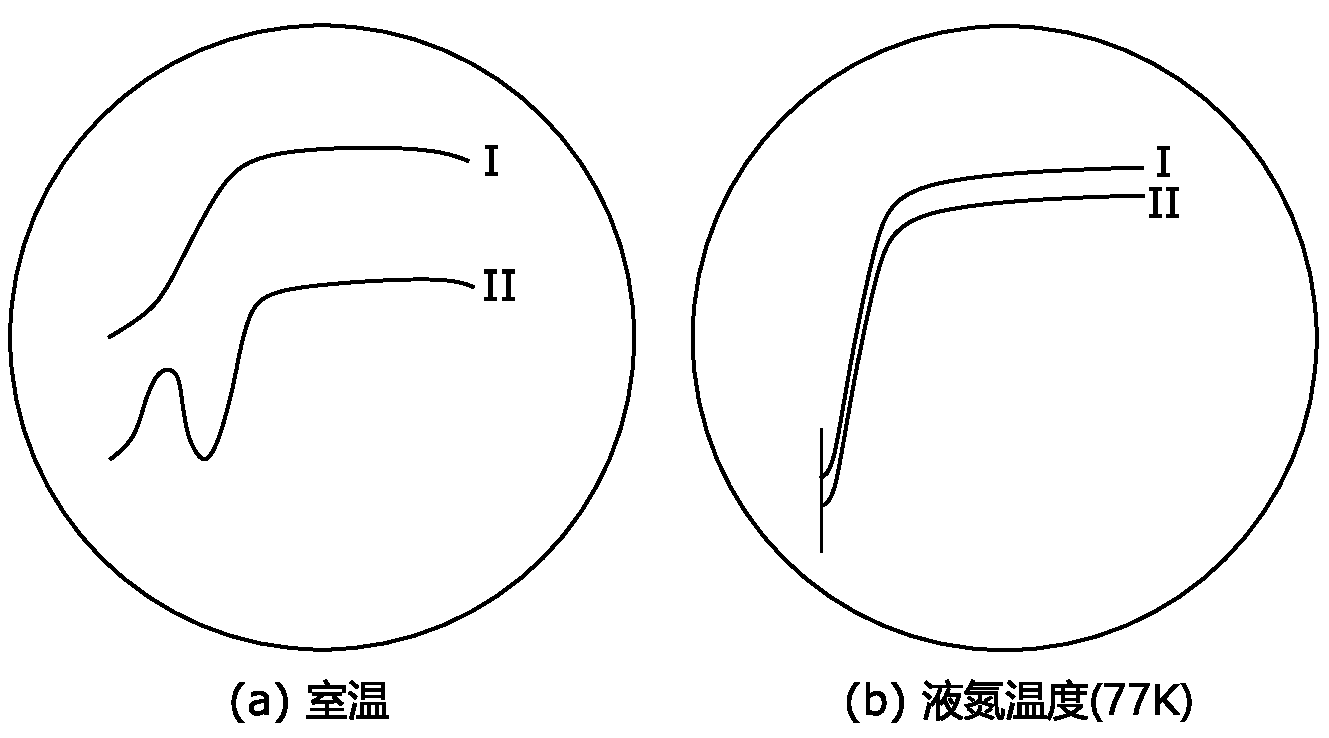
\includegraphics[width=0.8\textwidth]{fig/fig12.pdf}\\
\caption{交流定性观察}\label{fig12}
\end{figure}

\item 一只手扶住闸流管管座,另一只手旋松支架上的固定螺丝,小心地将闸流管玻壳缓慢移入装有液氮的保温瓶内,让管顶浸入液氮,切不可使金属管座接触液氮,否则会炸裂。

观察$I_C-V_A$曲线的变化,其凹陷消失。
\item 接触电势差的补偿:由于屏蔽极和板极间接触电势差的存在,碰撞空间不是等势空间。$V_A$很小时,$I_A$和$I_C$不同时出现。(必要时将X轴扫描扩展10倍,)仔细调节示波器$Y_1$和$Y_2$的放大倍数以及补偿电压$E_C$的值,使曲线\rom{1}和\rom{2}基本上全部重合,如图(\ref{fig12}-b)所示,此时可认为接触电势差得到补偿。以后操作保持$E_C$不变。
\end{enumerate}
\subsection{直流测量}
\begin{enumerate}
\item 连接线路。并关掉示波器。闸流管仍置于液氮中。选择好灯丝电压,将$V_A$调至较大负电压,使闸流管完全截止。两微电流计置于最小量程。
\item 测量液氮温度下一组$V_A$,$I_A^{\*}$,$I_C^{\*}$值,由于实验曲线以$\sqrt{V}$为横坐标,所以起始时$V_A$间隔应取得小些。
\item 将闸流管从液氮中取出,待温度平衡后,将$V_A$置1.00V左右,由于室温下氙原子的导热使阴极温度稍微下降,故应适当增加灯丝电压$V_F$,使室温下的$I_A+I_C$等于低温下的$I_A^{\*}+I_C^{\*}$,即保持阴极温度不变。然后取与低温下相同的$V_A$值,测量一组$I_A$,$I_C$值,根据测得的数据,计算可得散射几率$P_s$和散射截面Q。
%\item 选择三种不同的灯丝电压,分别测量$P_s-\sqrt{V}$曲线(选做)。
\end{enumerate}
\section{注意事项}
\begin{enumerate}
\item 处理液氮时要小心。不要装得太满;闸流管只要浸没一部分,不可使金属管座接触液氮,否则,管子容易炸裂。当用液氮进行测量时,先要关掉灯丝电源,直到把管子顶端浸入液氮后,再接通灯丝电源,这样做,管子破裂的机会就少。
\item $V_A$幅度增大到一定值,电流会出现急剧增加,这时需注意减少$V_A$,以防碰撞管电离。
\end{enumerate}

\section{实验数据}

\section{误差分析}

\section{思考题}
\subsection{已知标准状态下氙原子的有效半径为2$\times$10$^{-10}$m,按经典气体分子运动论计算其散射截面及电子平均自由程,再将实验所得$P_s$最小值和最大值对应的散射截面求出来,与经典结果作比较,并讨论之。}

\subsection{对示波器上显示的$I_A-V_A$与$I_C-V_A$曲线做出定性解释。}

\subsection{为何修正后的曲线上的第二、三、四数据点比预期偏低?}

\nocite{jiaocai}
\bibliography{ref}
\end{document}